%&pdflatex
\documentclass[xcolor=svgnames]{beamer}
\usepackage[british]{babel}
\usepackage[T1]{fontenc}

\usepackage{minted}

\usepackage{tcolorbox}
\usepackage{graphicx}
\usepackage{booktabs}

\usepackage{lmodern}

\usepackage{bytefield}

\useinnertheme{default}
\useoutertheme{infolines}
\usecolortheme{seahorse}
\setbeamercolor*{alerted text}{fg=blue!75!black}
\setbeamertemplate{blocks}[rounded]
\setbeamertemplate{itemize item}[triangle]
\setbeamertemplate{itemize subitem}[circle]
\setbeamertemplate{itemize subsubitem}[square]

\usecolortheme{rose}
\definecolor{NUblue}{RGB}{62,141,165}
\definecolor{NUbluedark}{RGB}{40,119,143}
\setbeamercolor*{palette primary}{use=structure,fg=white,bg=NUblue}
\setbeamercolor*{palette quaternary}{fg=white,bg=NUbluedark}
\setbeamercolor{section in head/foot}{fg=white,bg=NUbluedark}
\setbeamercolor{subsection in head/foot}{fg=white,bg=NUblue}
\setbeamercolor{frametitle}{fg=NUbluedark!150,bg=NUblue!40}
\setbeamercolor{title in head/foot}{fg=white,bg=NUblue}
\setbeamercolor{author in head/foot}{fg=white, bg=NUbluedark}
\setbeamercolor{date in head/foot}{fg=white, bg=NUblue!60}
\setbeamercolor{title}{fg=NUbluedark!150,bg=NUblue!30}
\setbeamercolor{date}{fg=NUbluedark!150}
\setbeamercolor{block title}{fg=white,bg=NUblue}

\usepackage{siunitx}
\usepackage{tikz-timing}
\usetikztiminglibrary{arrows}
\usepackage[european]{circuitikz}

\usetikzlibrary{graphs, fit, arrows.meta}

\title{Control systems and Computer Networks}
\subtitle{Discrete Time and Interrupts}

\author{Dr Alun Moon}
\date{Lecture 02.2}
\begin{document}
\frame{\maketitle}

\part{Inputs}
\frame\partpage

\begin{frame}{Time}
\begin{itemize}
  \item In the real world we have to deal with time.
  \item The CPU is driven by a clock signal\\
      \texttiming{20{C}}
  \item From the CPU point of view we can think of time as being
      in discrete chunks.
  \item External clock is \SI{50}{\mega\hertz}
  \item Cortex M4 core clock \SI{120}{\mega\hertz}
  \item Clock period $\sim\SI{8}{\nano\second}$
\end{itemize}
\end{frame}

\begin{frame}[fragile]{Polling}
  Consider the following code, polling the switch every \SI{100}{\milli\second}\\
  (10 times a second).
  \begin{exampleblock}{}
  \begin{minted}{c}
      while(1) {
        if( ispressed(SW1) ) action();
        wait(0.1);
      }
  \end{minted}
\end{exampleblock}
\begin{itemize}
  \item The GPIO circuit looks at the switch for \SI{10}{ns}
  \item We end up looking at the switch every \SI{10}{ns} out of every \SI{100}{ms}
  \item \alert{or} for 0.00001\% of the time.
\end{itemize}
\end{frame}

\begin{frame}{We can miss important events...}
  \begin{tikztimingtable}
      Polling & LL2{H15{L}}HLL \\
      Event   & L5{L}5{H}24{L}L \\
  \end{tikztimingtable}
\begin{itemize}
  \item If the event we are watching for is smaller that the time between polls.
  \item We can fail to spot the event entirely
\end{itemize}
\vspace{\fill}
\begin{tikztimingtable}
    Polling & LL2{H15{L}}HLL \\
    Event   & L35{H}L \\
\end{tikztimingtable}
\begin{itemize}
  \item For long events.
  \item When exactly is the button pressed?
\end{itemize}
\end{frame}

\begin{frame}{Interrupts}{Event driven programming}
\begin{itemize}
  \item Recall the \emph{fetch}-\emph{execute} cycle.\\
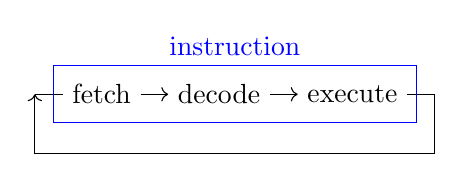
\begin{tikzpicture}
\graph[grow right sep] {
 p1[coordinate] -- fetch -> decode -> execute -- p2[coordinate];
 };
 \draw[->](p2) -- +(0,-0.75) -| (p1);
 \node[draw=blue, fit=(fetch) (execute), label={[blue]instruction}] {};
\end{tikzpicture}
\item Interrupts occur \emph{asynchronously}\\
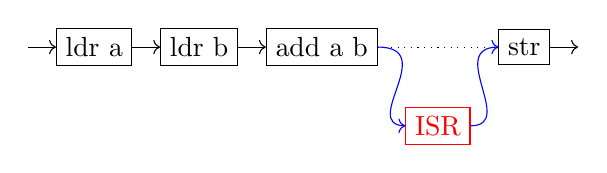
\begin{tikzpicture}[every node/.style={draw}]
  \graph[grow right sep] {
    o[coordinate] -> ldr a -> ldr b -> add a b -!- {irq[coordinate], ISR[red]} -!- str -> e[coordinate];
  };
  \draw[dotted] (add a b) -- (str);
  \draw[->,blue] (add a b) .. controls +(0:1.5cm) and +(180:1cm) .. (ISR);
  \draw[->,blue] (ISR) .. controls +(0:1cm) and +(180:1cm) .. (str);
\end{tikzpicture}
\item When an \alert{Interrupt} occurs (IRQ) the program jumps out of the normal flow,
  to the interrupt handler (ISR), then returns to the next instruction in the normal flow.
\end{itemize}
\end{frame}

\begin{frame}{Digital Inputs}{Edge triggered interrupts}
\begin{itemize}
  \item with a digital signal where do we raise an interrupt request?\\
    \texttiming[x=3\xunit,y=2\yunit]{LLHLL}
    \item The easiest thing to do, is to detect \alert{changes} in the signal
    \begin{description}
      \item[Rising Edge] the signal goes from 0 to 1\\[1em]
      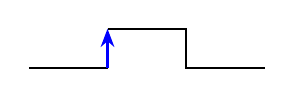
\begin{tikzpicture}[>=Stealth]
        \draw[thick] (0,0) -- (1,0);
        \draw[thick,blue,->] (1,0) -- (1,0.5);
        \draw[thick] (1,0.5) -- (2,0.5) -- (2,0) -- (3,0);
    \end{tikzpicture}\\[2em]
      \item[Falling Edge]      the signal goes from 1 to 0 \\[1em]
      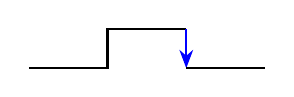
\begin{tikzpicture}[>=Stealth]
              \draw[thick] (0,0) -- (1,0) -- (1,0.5) -- (2,0.5);
              \draw[thick,blue,->] (2,0.5) -- (2,0);
              \draw[thick] (2,0) -- (3,0);
          \end{tikzpicture}

    \end{description}
\end{itemize}
\end{frame}

\begin{frame}[fragile]{Interrupt Service Routines}
\alert{ISR}s cannot take parameters or return values
    \begin{block}{ISR prototype}
    \begin{minted}{c}
      void buttonISR( void );
    \end{minted}
  \end{block}
  Any data that needs to be passed between the ISR and the program needs to be done
  via \emph{global variables}\\[1em]

\alert{ISR}s need to be kept short.  Remember the code is executing \emph{between} other instructions.\\
\alert{Avoid} slow operations such as reading and writing to the display or serial port.

\end{frame}

\begin{frame}[fragile]{Creating an Inturrupt handler}
\begin{exampleblock}{}
\begin{minted}{c}
    InterruptIn  left(SW2);
    InterruptIn right(SW3);

    left.rise(on);
    right.fall(off);
    while(1) /* GNDN */ ;
\end{minted}
\end{exampleblock}
\begin{itemize}
\item Only some pins can generate interrupts
\item an action can be attached to rising and falling edges
\item \alert{Remember} to check for logic inversions (pressed is a falling edge)
\item Actions occur \emph{independently} from the \emph{main-loop}
\end{itemize}
\end{frame}

\part{Timers}
\frame\partpage


\begin{frame}[fragile]{Timeing }
\begin{itemize}
\item For many applications we want something to happen periodically
\item using loops and delays is problematic
\begin{minted}{c}
while(1) {
    int sensor = ispressed(SW1);
    printf("button is %s presesed", sensor?"":"not" );
    wait(1);
}
\end{minted}
\item Timing depends on execution time of code.
\begin{itemize}
\item difficult to predict
\item varies from loop to loop
\end{itemize}
\end{itemize}
\end{frame}


\begin{frame}{Periodic Interrupt Timer}
\begin{itemize}
\item We can generate interrupts from a hardware timer
\item these can be set at a particular period
\item an IRQ is generated an each period.
\item Accurate precise times
\begin{itemize}
\item lower resolution -- the system clock $\sim\SI{8}{ns}$
\item upper bound -- when the counter rolls over \SI{34}{s} for 32 bits
\item for 4 chained timers \SI{2.7e30}{s} (\SI{8e22}{a} or \SI{6e12}{universe})
\end{itemize}
\end{itemize}
\end{frame}

\begin{frame}{Using a PIT}{Soft timers}
\begin{itemize}
\item Once we have a periodic \emph{tick}
we can do interresting things
\item the ISR can count \emph{tick}s
\begin{exampleblock}{On tick}
\begin{description}
\item[0] LED on
\item[2] LED off
\item[5] reset tick to 0
\end{description}
Turns the LED on for  $2/5$ of the time
\end{exampleblock}
\end{itemize}
\end{frame}

\begin{frame}[fragile]{MBed}
The MBed library uses a single soft-timer to handle PIT interrupts
\begin{minted}{c}
  Ticker pit;
  pit.attach(flash,0.5);
  while(1);
\end{minted}
\begin{itemize}
\item Attaches the \texttt{flash} function to be called every \SI{0.5}{s}
\item Happens independently to main-loop
\item Concurrency!  (without the messing about with OS)
\item Library supports any number of PIT interrupts
\end{itemize}

\end{frame}

\begin{frame}{Interrupt timing}{The fine details}
\begin{itemize}
\item There is a delay between the IRQ being raised and the ISR starting.
\begin{tikztimingtable}
IRQ & LG20L \\
`main' execution & U4U10L6U \\
ISR & 5L{[red,fill=red!50] 8U}8L \\
Interrupt latency & L4H16L \\
\end{tikztimingtable}
\item Remember not to make ISRs too long
\begin{tikztimingtable}
IRQ & L3{G10L} \\
Bad & L{[red,fill=red!50]15U}15L\\
Good &L3{{[red]5U}5L} \\
\end{tikztimingtable}
\end{itemize}

\end{frame}

\end{document}
